\documentclass[11pt]{article}
%Gummi|065|=)
\title{Homework \#1: Discussion on the Cosine, \\ Jaccard, and Euclidean Similarities\\ of CNN News Articles}
\author{Doug McGeehan\\
		CS 6001: Applied Spatial and \\ Temporal Data Analysis\\
		Spring 2017}

\usepackage[margin=1in]{geometry}
\usepackage{verbatim}
\usepackage{framed}
\usepackage{amsmath}
\usepackage{amssymb}
\usepackage{graphicx}


\begin{document}

\maketitle

\section{Introduction}

In this report, an analysis of 100 news articles is performed whereby every pair of articles is compared with one another to determine their similarity.
The metrics in which similarity is computed are through the cosine similarity, Euclidean distance, and Jaccard similarity of the term-frequency vectors of each article.
A custom-written software package was implemented in the Python 3 programming language so as to perform this analysis and visualize the results.
The findings from this analysis indicate that the cosine similarity is the best suited similarity metric for identifying articles covering similar semantic topics, with the Jaccard similarity following close after.
Euclidean distance, on the other hand, performs quite poor, exhibiting bias towards pairs of short articles.

The outline of this paper is as follows.
Section \ref{sec:dataset} discusses the news article dataset used in this analysis.
Section \ref{sec:software} gives a brief summary of the implementation details of the software used to perform similarity analysis.
Finally, Section \ref{sec:experiments} explains the experimental setup and discusses findings from these experiments, followed by closing remarks in Section \ref{sec:conclusion}.


\section{News Article Dataset} \label{sec:dataset}

For this report, a dataset consisting of over 2000 articles from CNN.com was chosen, with articles spanning January 1st, 2014 to April 4th, 2014\footnote{
https://sites.google.com/site/qianmingjie/home/datasets/cnn-and-fox-news
}.
This dataset was compiled by Qian and Zhai for their research in multi-view unsupervised feature selection on unlabeled text and image data \cite{qian2014unsupervised}.
Articles within the dataset span multiple categories, such as crime, politics, and entertainment.
The number and proportion of articles to each category is provided in Table \ref{tab:categories}.

\begin{table}[h]
	\centering
	\begin{tabular}{ r c c c c  }
		\hline
	Category: &              Politics & Entertainment & Crime & \\ \hline
	Number of Articles: &    409 &      392 &           349 & \\ \hline
	Percentage of Dataset: & 20\% &    19\% &           17\% & \\
	  \hline
	  \hline
	   Health & Travel & Living & Technology \\ \hline
	   286    & 273    & 198    & 148 \\ \hline
	   14\%   & 13.3\% & 10\%   & 7.2\% \\
	\hline
	\end{tabular}
	
	\caption{Number and Proportion of Articles per Category}
	\label{table:categories}
\end{table}


\subsection{Article Contents}

For this report's experiments, the images accompanying each article were discarded and only the textual portion of the articles was analyzed.
Each article is represented as an XML document with tags corresponding to the article's content and metadata.
Of interest is the content within the \texttt{<TEXT></TEXT>} block.
Everything else is ignored.

\pagebreak
\subsection{Example of an Article}

\small 
\begin{quote} \label{samplearticle}
\begin{verbatim}
<DOC>
    <DOCNO>1897</DOCNO>
    <URL>
        http://rss.cnn.com/\~r/rss/cnn\_allpolitics/\~3/
        -AmYNL5GUcc/index.html
    </URL>
    <TITLE>
        Obama to Iran: 'We have the opportunity to start
        down a new path'
    </TITLE>
    <TIME>Thu, 20 Mar 2014 11:10:42 EDT</TIME>
    <ABSTRACT>
        In a message to the Iranian people, an upbeat President
        Barack Obama said Thursday that the long isolated
        Middle East nation can soon improve its economy, its
        world standing and its people's lives if there's a
        breakthrough nuclear deal.
    </ABSTRACT>
    <TEXT>
        (CNN) -- In a message to the Iranian people, an upbeat
        President Barack Obama said Thursday that the long
        isolated Middle East nation can soon improve its
        economy, its world standing and its people's lives if
        there's a breakthrough nuclear deal.
        ...
    </TEXT>
</DOC>
\end{verbatim}
\end{quote}
\normalsize

%\begin{Verbatim}[frame=single]
%\end{Verbatim}

\section{Implementation} \label{sec:software}

Custom-written software was developed for the purpose of performing the experiments of this report. This software was written in the Python 3 programming language and the HTML5 markup language and performs such tasks as automatic extraction of the dataset, corpus transformation into a term-frequency matrix, pairwise article similarity computation, and the presentation of the final sorted results in both an easy to read textual format as well as a web page.
There were many external libraries used to facilitate this functionality.
These libraries are summarized in Table \ref{tab:libraries}.

\begin{table}[h] \label{tab:libraries}
	\centering
	\begin{tabular}{ r|c|l }
		\hline
		Environment: & Library & Purpose \\ \hline
		Python: & BeautifulSoup & Parsing the XML of the news articles \\
		&	scikit-learn\cite{scikit-learn} & Corpus to term-frequency matrix transformation \\
		& & and stopword filtering \\
		& 	SciPy\cite{scipy} & Euclidean and Cosine distances \\
		&   numpy & Fast vector operations \\
		&  pickle & Fast reloading of experiment results \\
		& matplotlib & Bar graphs and other visual aids \\ \hline
		Webpage & Bootstrap & Simplified gridwork and design \\
		&  Flask  & Lightweight web server for Python \\
		& Jinja & Web page templating for Python
	\end{tabular}
	
	\caption{Software Libraries and Technologies used in the Software Implementation}
\end{table}

\subsection{Distance Metrics}

The SciPy project \cite{scipy} offers many distance functions operating on a pair of vectors as part of their spatial module\footnote{
https://docs.scipy.org/doc/scipy/reference/spatial.distance.html
}, including one for Euclidean distance %\footnote{
%https://docs.scipy.org/doc/scipy/reference/generated/scipy.spatial.distance.euclidean.html
%}
and Cosine distance. %\footnote{
%https://docs.scipy.org/doc/scipy/reference/generated/scipy.spatial.distance.cosine.html
%}
These functions compute various \emph{dissimilarity} metrics which require mapping to an appropriate similarity metric.
Details on this mapping is provided in Section \ref{sec:mapping}. 

Although there is a distance function named \texttt{jaccard}, it does not compute the Jaccard similarity, but rather the Jaccard-Needham dissimilarity\footnote{
https://docs.scipy.org/doc/scipy/reference/generated/scipy.spatial.distance.jaccard.html
} which cannot be directly mapped to a Jaccard similarity.
Thus, a custom-implemented Jaccard similarity function was developed for this report.
Given two $n$-dimensional vectors $\hat{u} = [ u_1, \cdots, u_n ]$ and $\hat{v} = [ v_1, \cdots, v_n ]$, where $u_i, v_i \ge 0 \, \forall \, 1 \le i \le n$, the Jaccard similarity metric, as is implemented in the custom-implemented Jaccard similarity function, is defined as:

\begin{equation} \label{eq:jaccard}
	s_{\text{jaccard}} = \frac{ \left| \{i \, | \, u_i = v_i \land u_i \ne 0 \} \right| }
	                          { \left| \{i \, | \, u_i = v_i \land u_i = 0 \}^\complement \right| }
\end{equation}
In relation to this report, the Jaccard similarity records the number of times in which one article has the same positive number of occurrences of a particular word as the other article.
This is then scaled by the number of unique words in the union of the two articles. For example, if two articles have the word ``beef'' occur 5 times, then it will be counted in the numerator of Equation \ref{eq:jaccard}.
However, if one article has the word ``dog'' 4 times and the other 3 times, it will not be counted in the numerator, but will be counted in the denominator.
Similarly, the abscence of a word in both documents (i.e. $\exists \, i$ such that $u_i = v_i = 0$) is not counted in either the numerator or the denominator.

For details on the definition of the Euclidean distance and the Cosine distance of two vectors, refer to the SciPi API reference in the footnotes on the previous page.

\subsection{Mapping Distance to Similarity} \label{sec:mapping}

In order to properly use distance metrics as a means to quantify the similarity between two vectors, the distance metrics need to be mapped to some value in the range $[0, 1]$ such that a value near 0 indicates the two vectors have low similarity, and similarity a value near 1 indicates high similarity.
The method in which the distance metrics were normalized is described below.

Let $d_i(u, v)$ denote the distance of vectors $u$ and $v$ as computed by the $i$-th distance method, and let $s_i(u, v)$ denote their corresponding similarity.
For Euclidean distance, the following formula is adopted to map it to a Euclidean similarity:

\begin{equation} \label{eq:euclid}
s_{euclid}(u, v) = \frac{1}{d_{euclid}(u, v) + 1}
\end{equation}
and for cosine distance:
\begin{equation} \label{eq:cosine}
s_{cos}(u, v) = 1 - d_{cos}(u, v)
\end{equation}
The Jaccard similarity was implemented as a similarity metric, and thus there is no need for a mapping.


\section{Experimental Setup and Analysis} \label{sec:experiments}

In this section, the results of the similarity analyses is reviewed and discussed.
The software described in Section \ref{sec:software} was executed on a randomly-selected subset of 100 articles from the CNN.com dataset compiled by Qian and Zhai \cite{qian2014unsupervised}.
These articles were transformed into a $100 \times n$ term-frequency matrix $C = [ c_{i,j} ]$, where $n$ is the total number of unique words in the union of all 100 articles, and $c_{i,j}$ represents the number of occurrences of the $j$-th word in the $i$-th article (i.e. $c_{i,j} \ge 0$ for $1 \le i \le 100$ and $1 \le j \le n$).


\subsection{Visualizing the Results}

Several plots and visual aids were created to assist in visualizing the results of this experiment.
Figure 1 demonstrates the pervasiveness of certain words, called stopwords, that offer minimal semantic relevance to the overall topic of a discourse.
More on this is discussed in Section \ref{sec:stopwords}.

To further assist with understanding the results of these experiments, a webpage was developed with the pairs of articles sorted by their similarity scores.
A screenshot of this webpage is given in Figure 2.
This webpage offered hints as to the underlying performance of each similarity metric, spawning the creation of more figures.
At the end of this report is Figure 6, which plots the sum of the article lengths for each pair, ordered by the ranking of the article for a particular similarity metric.
This figure is particularly intriguing, and its results will be discussed later on in this section.


\begin{figure}[h] \label{fig:stopwords}
  \centering
  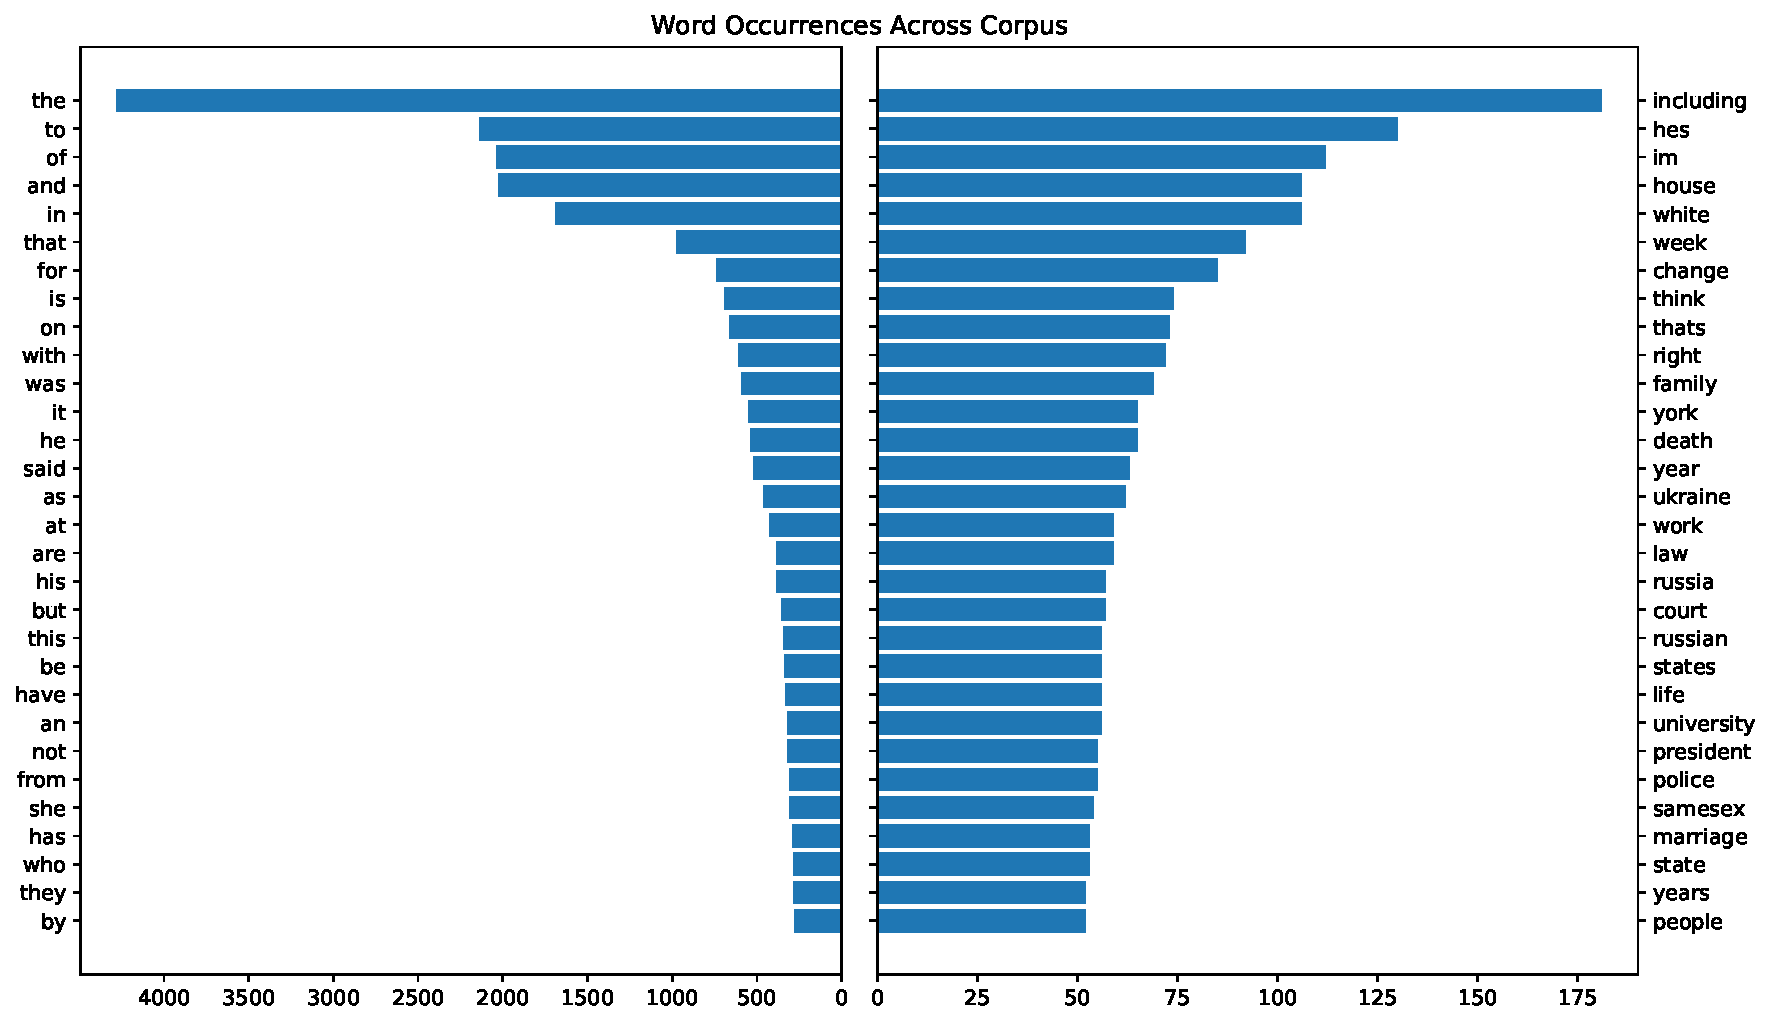
\includegraphics[width=\textwidth]{figures/stopwords}
  \caption{The 30 most frequent words in the corpus. The left panel shows a high occurrence of stopwords which offer little semantic meaning. The right panel shows the most frequent words after stopwords defined by the Glasgow Information Retrieval Group were removed.}
\end{figure}

\subsection{Stopwords: Filtering out Semantically Meaningless Words} \label{sec:stopwords}

In the English language, there are some of words that occur disproportionally frequent in dialog and written texts.
A few examples include ``the'', ``a'', ``among'', ``nevertheless'', and ``indeed''.
Indeed, the presence of these words skew the results of these experiments because of their frequent reoccurrence.
These are called stopwords and are typically filtered out before or after processing natural language data.
Figure \ref{fig:stopwords} illustrates the most frequently occurring words in the selected 100-article corpus before (left) and after (right) stopwords are removed.

To prevent stopwords from interferring with the similarity experiments of this report, and to accommodate meaningful comparisons between articles, the words occurring more than 300 times were removed from the term-frequency matrix.
Additionally, words that were defined as stopwords by the Glasgow Information
Retrieval Group\footnote{http://ir.dcs.gla.ac.uk/resources/linguistic\_utils/stop\_words} were also removed.
As indicated in the right panel of Figure 1, there still remains many stopwords in the corpus, such as ``including'', ``he's'', and ``that's''.
Due to time constraints, the list of all present stopswords was not completely constructed.


\begin{figure}[h] \label{fig:website}
  \centering
  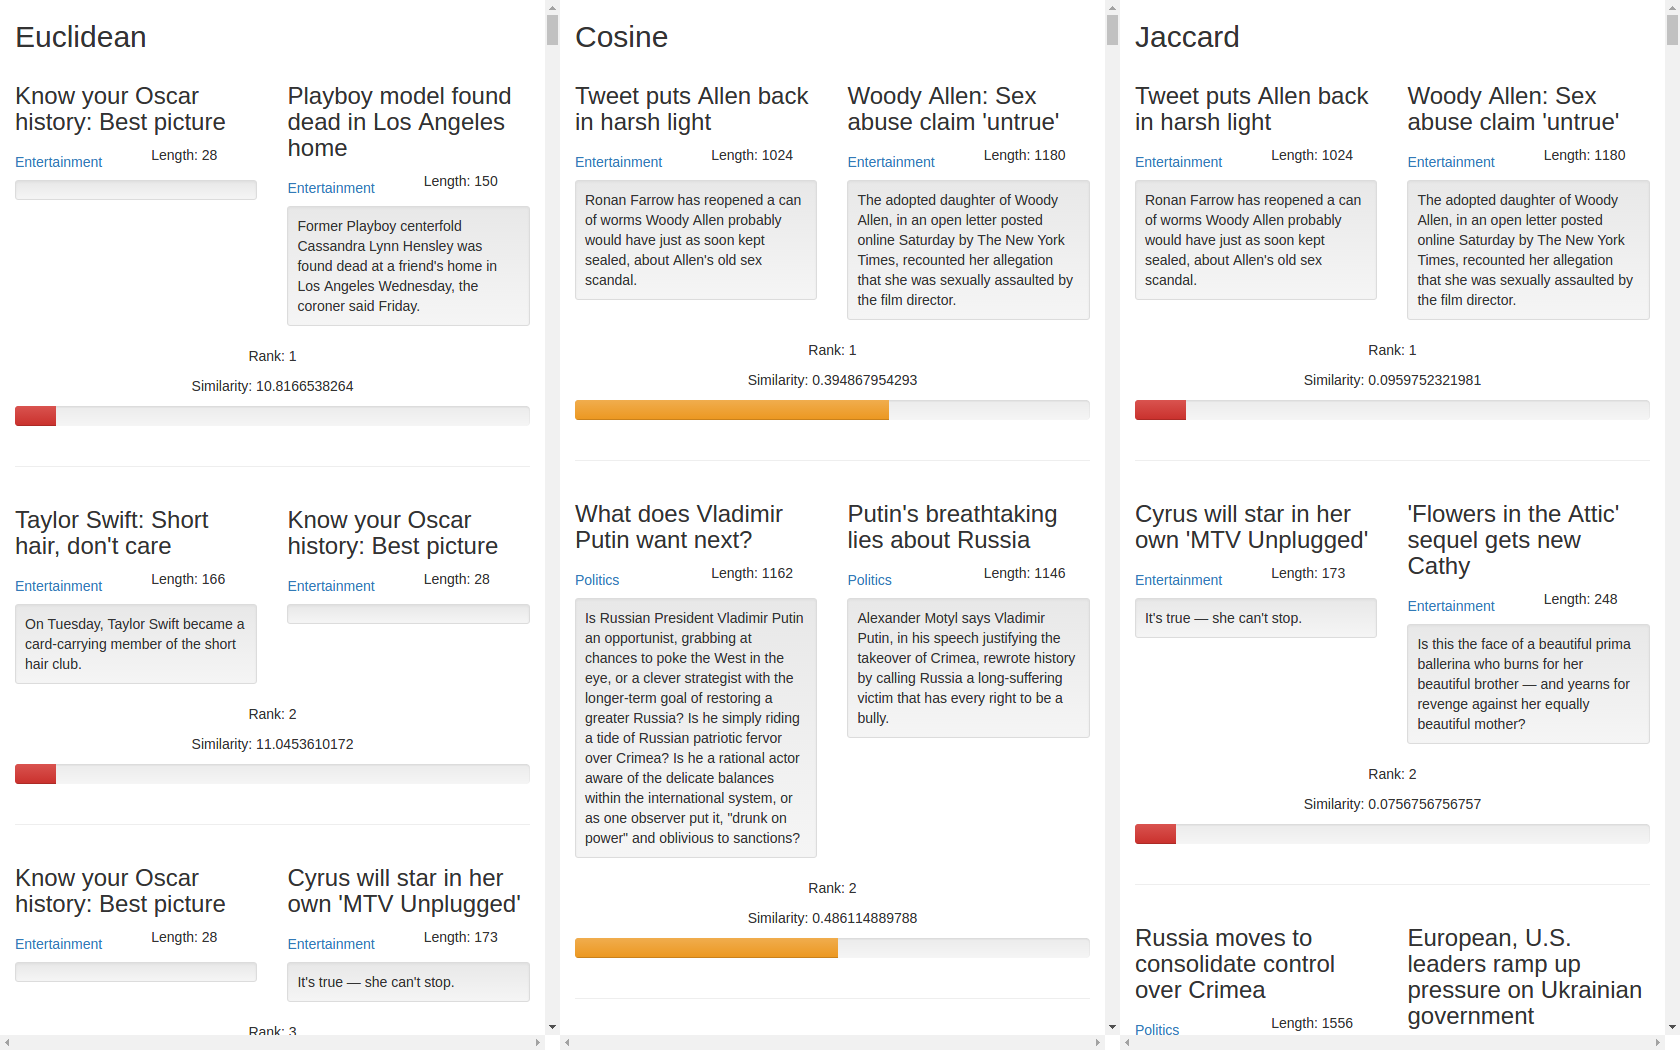
\includegraphics[width=\textwidth]{figures/webpage}
  \caption{A webpage was developed to assist with analyzing the results of this experiment.
  The page was split into three columns, one for each similarity metric.
  Each pair of articles is then sorted in descending order of their similarity scores.
  To assist in determining which metric offered the best results for semantic grouping, each article entry is also accompanied by the article's abstract and a link to the article's content for further reading.}
\end{figure}

\subsection{Results of Euclidean Distance}

\begin{figure}[h] \label{fig:euclid}
  \centering
  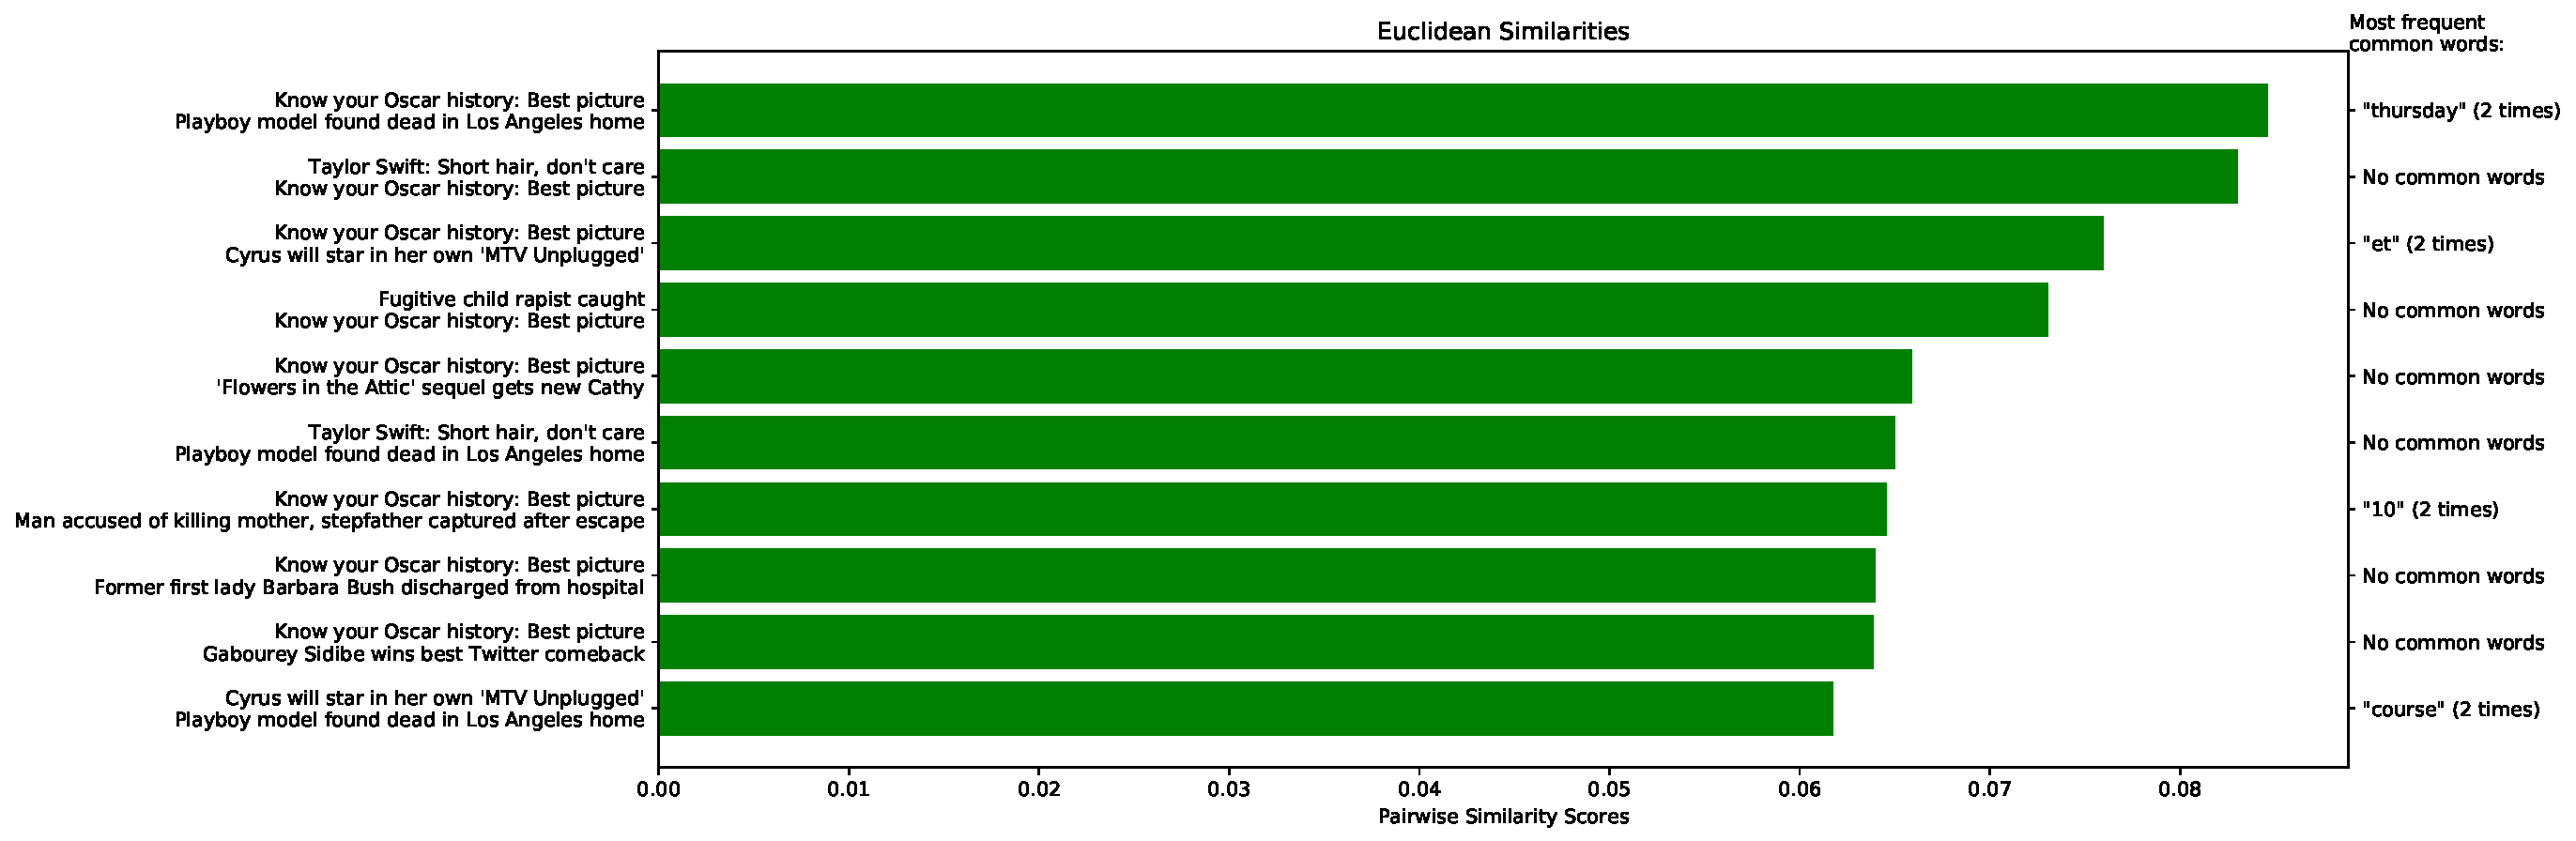
\includegraphics[width=\textwidth]{figures/euclidean_most_sim}
  \caption{The top 10 article pairs with the highest Euclidean similarity.
  The right-side axis shows the word that had the most common occurrence in both documents.}
\end{figure}

The use of the Euclidean Distance, as normalized by the Equation \ref{eq:euclid}, shows bias towards pairs of short articles and appears to perform poorly at grouping semantically similar articles together.
This is most strikingly illustrated in Figure 6 at the end of this report, whereby there is a significant correlation between the similarity between a pair of articles and the sum of their word counts.
Intuitively, these articles have tokenized vectors filled with the most zeros and the lowest article lengths as compared with other articles.
This results in a small Euclidean distance between two vectors, as both vectors are closer to the origin of the corpus' word space than longer documents, and thus much closer to one another.

The poor performance of the Euclidean distance is also demonstrated in Figure 3, which provides a list of the top 10 article pairs with the highest Euclidean similarity between one another.
This figure demonstrates that there are many repeats of the same article reappearing in higher rankings.
For example, the article titled "Know your Oscar history: Best picture" appears 8 times out of 10.
The flaws in the Euclidean distance becomes even more apparent when one analyzes the common words shared between two documents with the lowest Euclidean distance.
Of the closest 10 pairs of documents, 6 share no words in common.


\subsection{Results of Jaccard Similarity}

Like the Euclidean distance, the Jaccard similarity shows some initial favoritism towards pairs of short documents, but not to the same extent.
From analysing the results depict on this project's webpage, 7 of the top 30 most similar article pairs had fewer than 500 words, which is lower than that of the Euclidean distance experiment.
This bias may be due to the Jaccard similarity's use of the total number of unique words as a normalizer of number of shared word observations.
For example, consider one pair of articles with 20 unique words, 5 of which appear the same number of times in both articles.
It's Jaccard similarity would be equal to $\frac{5}{20} = 0.25$.
For a pair of articles with 500 unique words, 5 of which having the same occurrence count, the Jaccard similarity would be equal to 0.01.
This is only a slight favoritism, though.
Of those same 30 articles, 20 of them have 700 or more words each.
As illustrated in Figure 6, the article lengths begin to scatter without any apparent correlations, thus demonstrating that this is not a defining characteristic of the Jaccard similarity.

\begin{figure}[h] \label{fig:jaccard}
  \centering
  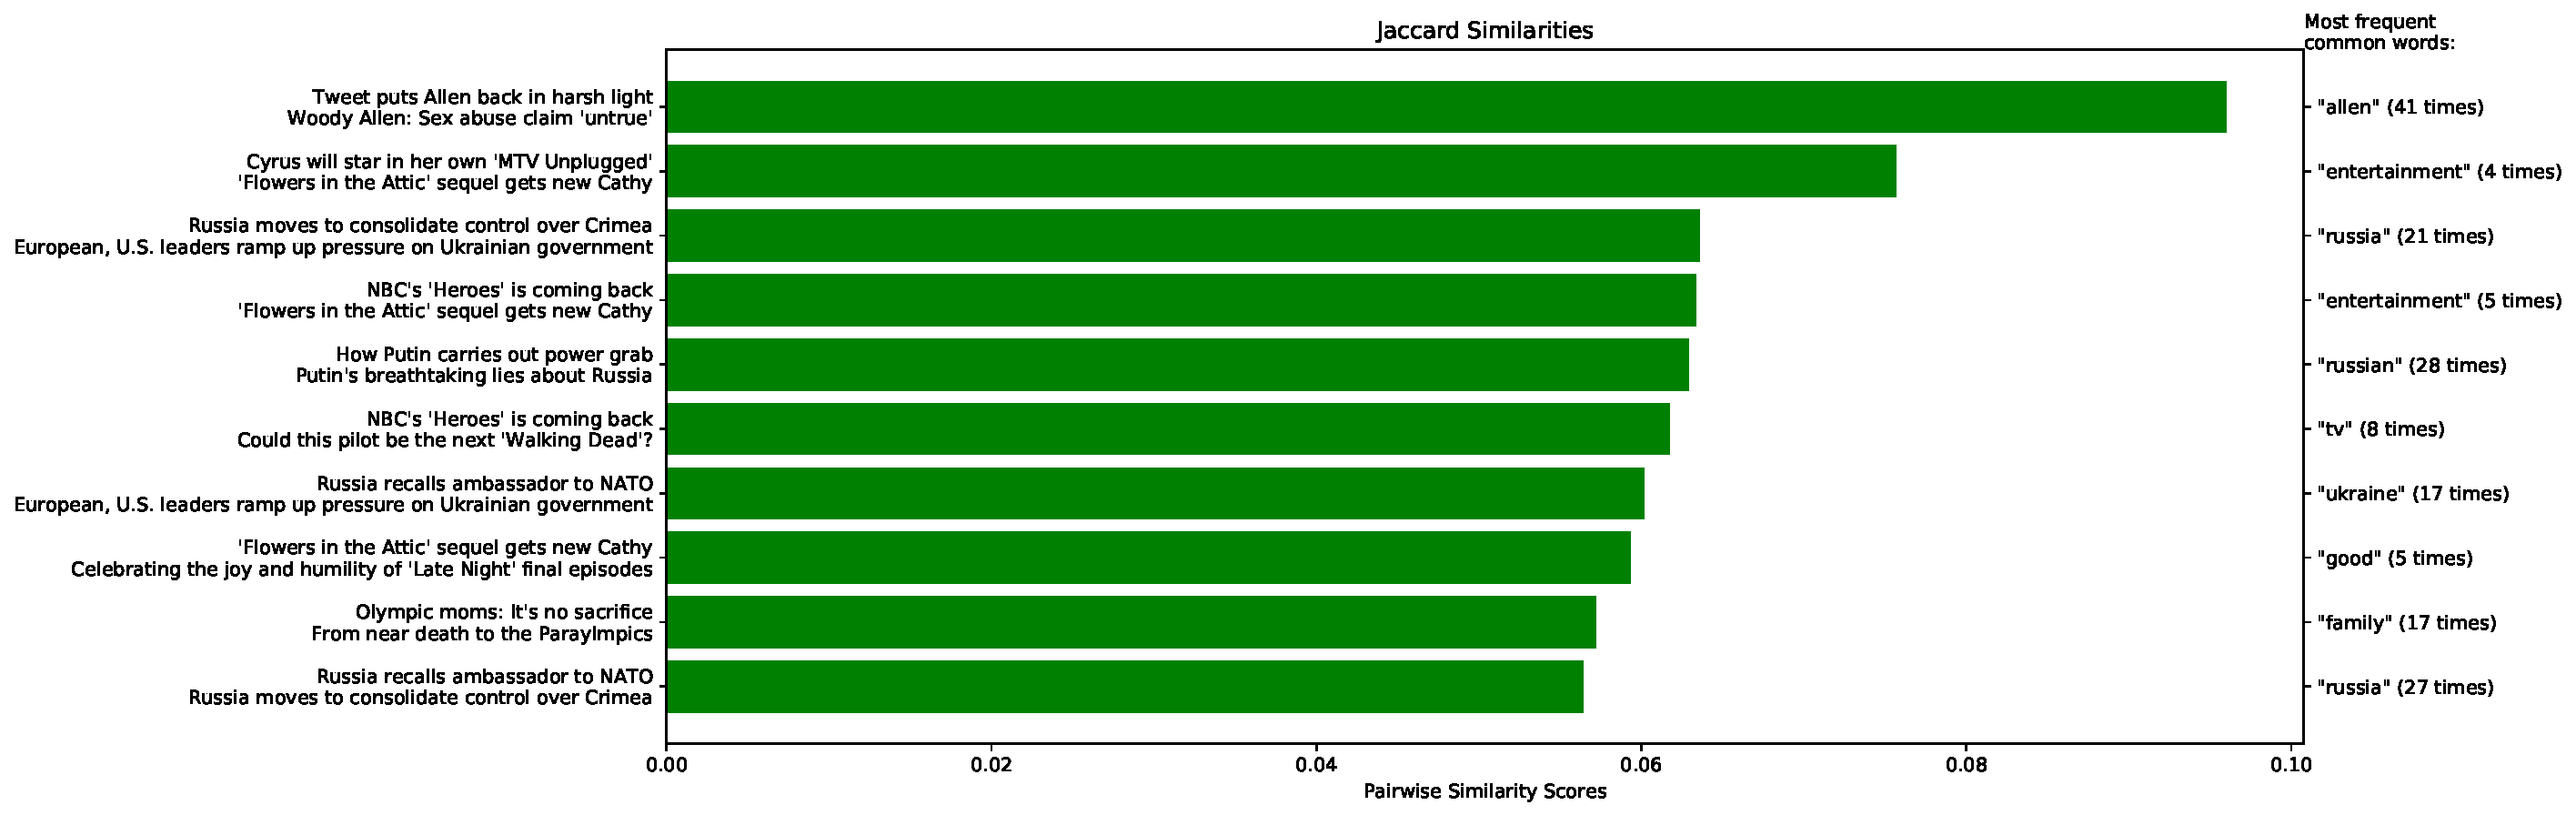
\includegraphics[width=\textwidth]{figures/jaccard_most_sim}
  \caption{The top 10 article pairs with the highest Jaccard similarity.}
\end{figure}

Unlike the Euclidean distance, those articles with the highest similarity appear to share semantic topics with one another.
For instance, the article pair with the highest Jaccard similarity discusses a scandal involving the actor and filmmaker Woody Allen, and the third most similar pair discusses Russia's involvement in Ukraine during the Crimea annexation.
As depicted in Figure 4, the titles of the top 10 article pairs indicates that it is partially successful in calculating similarities effectively.
However, there are false positives in the list mainly attributed to pairs of articles with fewer than 500 words.

\subsection{Results of Cosine Distance}

\begin{figure}[h] \label{fig:cosine}
  \centering
  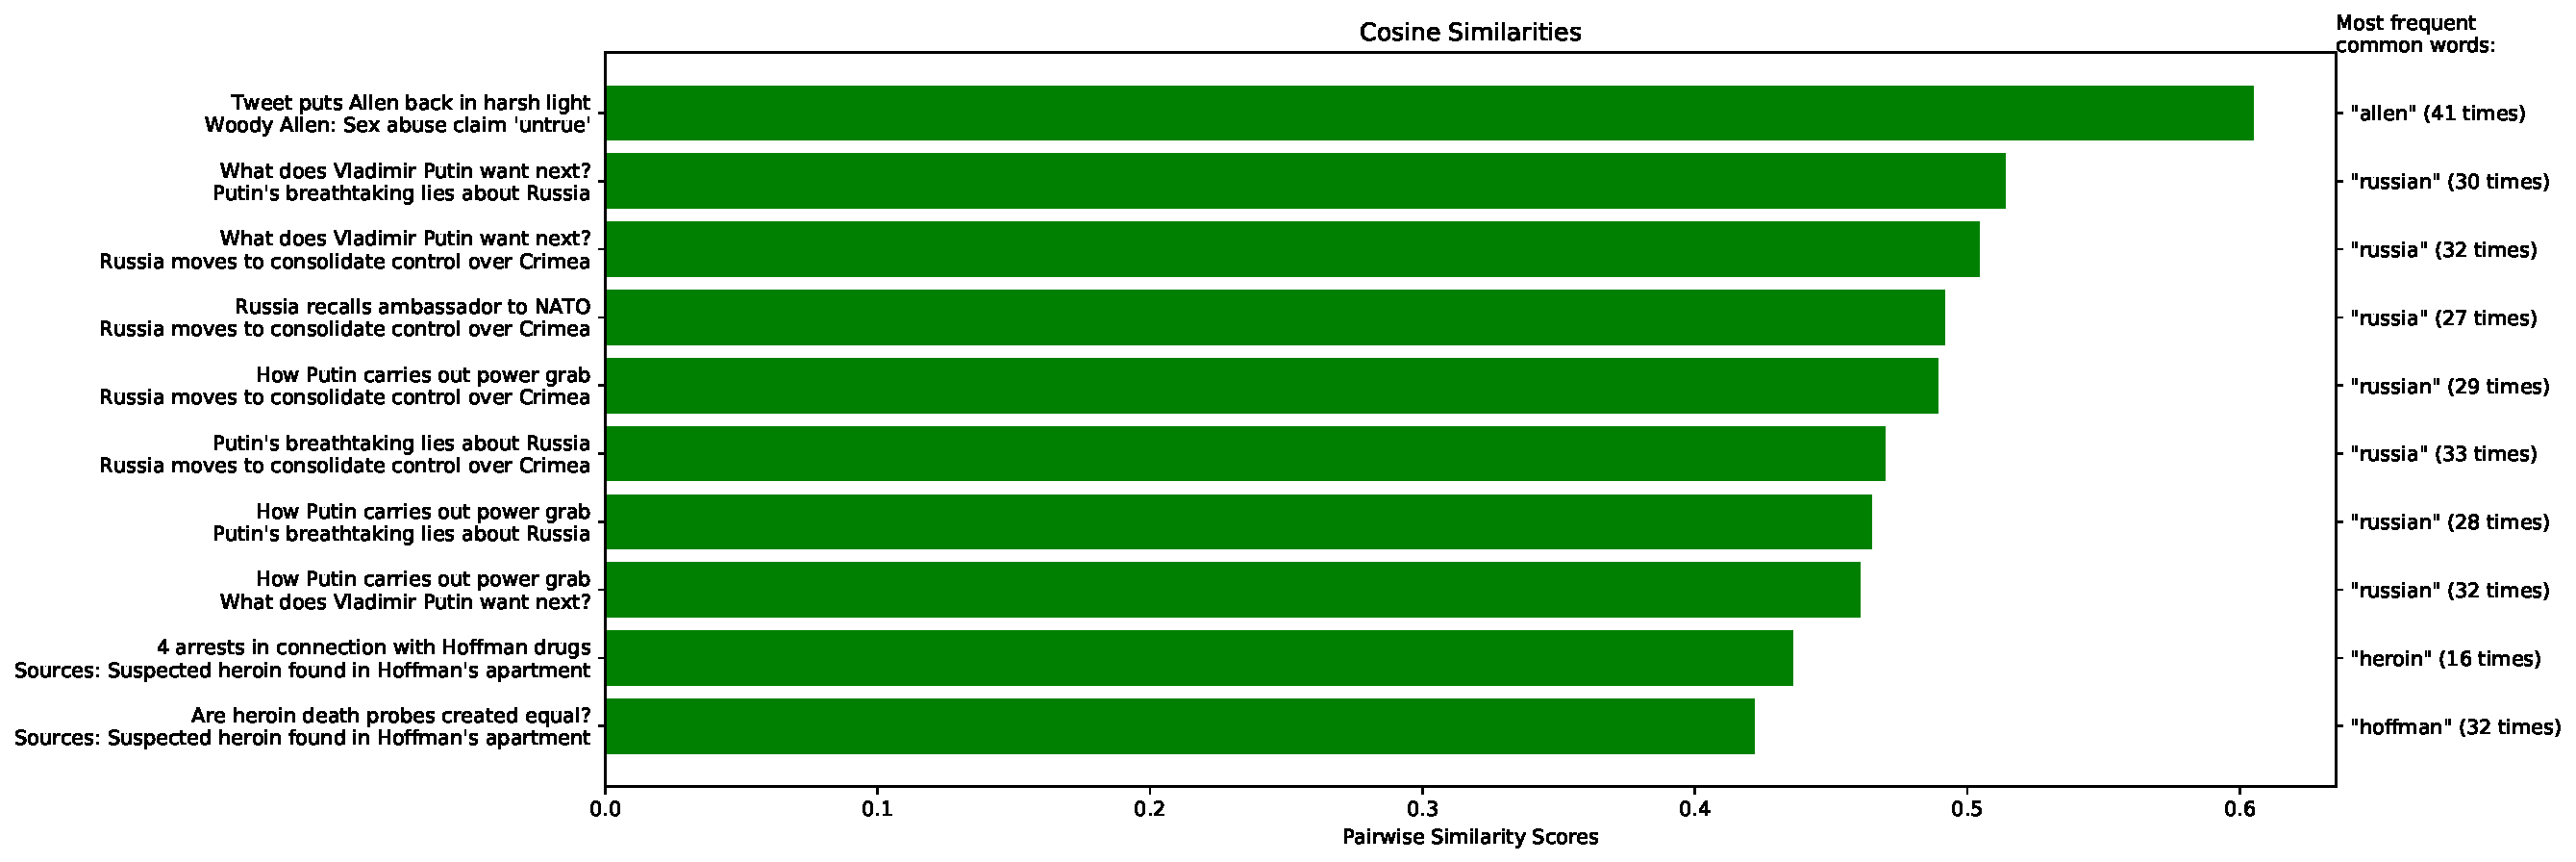
\includegraphics[width=\textwidth]{figures/cosine_most_sim}
  \caption{The top 10 article pairs with the highest Cosine similarity.}
\end{figure}

Figure 5 lists the top 10 article pairs that garnered the highest cosine similarity.
The benefit of the Cosine distance is that it doesn't show bias towards short documents as do the Jaccard similarity and Euclidean distance metrics.
This is due to its usage of the angle between two article vectors as opposed to their cardinality and length, respectively.
If two articles share many of the same words, they will point towards the same region in the corpus' word space and thus have a small angle between them, regardless of the vector's magnitude.
This trait offers an improvement on its ability to identify semantically similar articles over that of the Jaccard similarity.
With the Jaccard similarity, as applied to term-frequency vectors, a shared word is only counted if and only if the word occurs the same number of times in one document as it does in the other.
Intuitively, this results in many false negatives, as semantically similar articles may not have a semantically meaningful word occur the same number of times in both articles.

The results from the Cosine distance show many of the same article pairs obtaining high similarity scores as those in through the Jaccard similarity. For instance, the first and second highest article pairs are on the Woody Allen scandal and Russia's involvement in Ukraine, respectively.
In regards to false positives, the Cosine distance appears to have the lowest of the three.
All of the top 30 ranking article pairs appear to share a similar semantic topic of discussion.

\section{Conclusion} \label{sec:conclusion}

Between the Jaccard similarity, cosine distance, and Euclidean distance, the results of a pairwise similarity analysis of 100 randomly selected news articles suggest that cosine distance is the best metric for identifying similar articles represented by term-frequency vectors.
However, there are a few instances where the two articles are not in equal tone. For instance, the 32nd ranking article pair primarily focuses on universities, but whereas one discusses notable university buildings in regards to their architectural beauty, the other discusses the death of a student due to a school shooting.
Although this result may be an outlier, it demonstrates the necessity of multiple tools in one's tool belt when performing feature extraction and document similarities.

For future investigations, an appropriate next step would be to use a term-frequency, inverse-document-frequency (tf-idf) matrix and to perform a comparative analysis with a term-frequency matrix approach.
The code for performing such an experiment has already been written, but due to time constraints an analysis of the results was omitted from this report.

\begin{figure}[h] \label{fig:articlelengths}
  \centering
  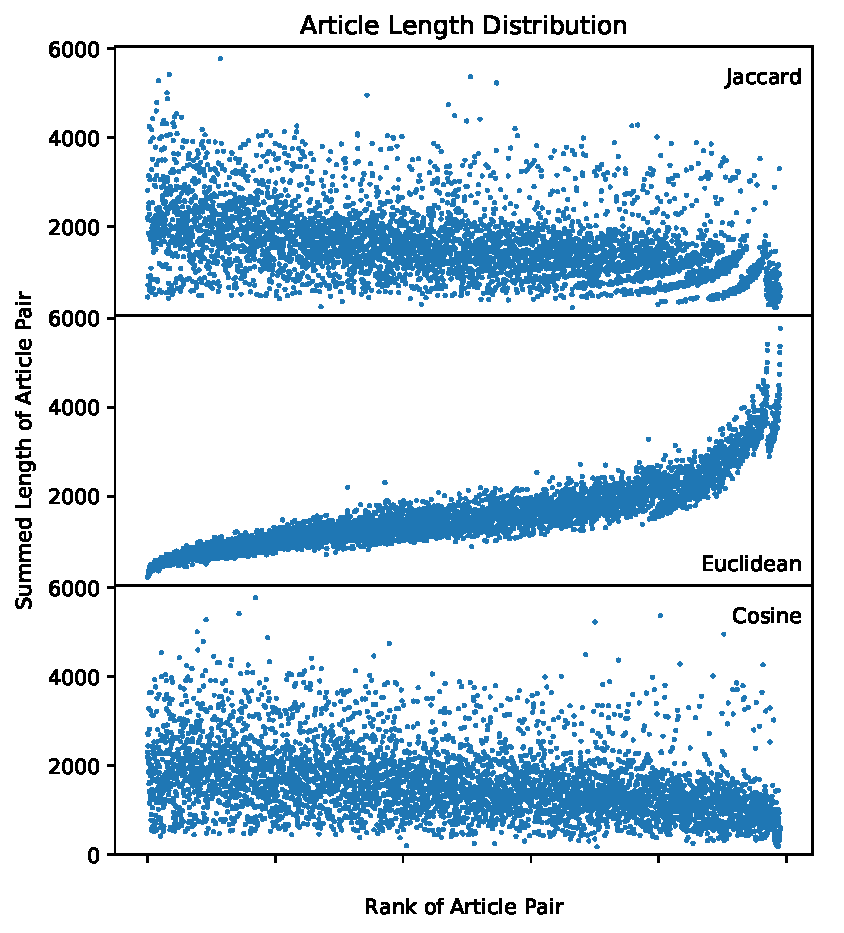
\includegraphics[width=\textwidth]{figures/article_length_dist}
  \caption{The summed lengths of each pair of the articles is plotted to demonstrate the bias towards short articles characteristic of the Euclidean distance. The opposite appears to be true for the Cosine and Jaccard similarity metrics.}
\end{figure}

\bibliography{bibliography}{}
\bibliographystyle{plain}
\end{document}
